\frametitle{Theory of refraction index}
\begin{minipage}{0.35\textwidth}
    \begin{figure}[h]
    \centering
    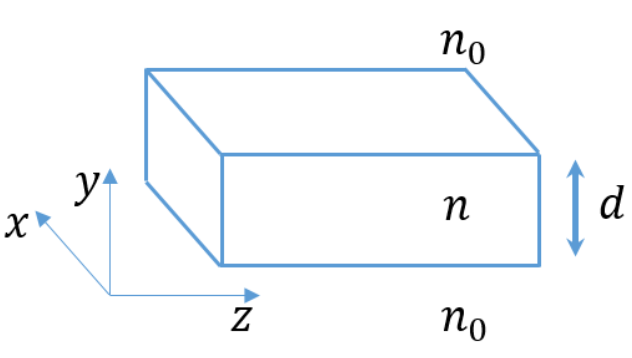
\includegraphics[width=1\textwidth]{images/nature_scheme.png}
    %\label{fig:}
\end{figure}
\end{minipage}
\hfill
\begin{minipage}{0.55\textwidth}
	The Helmholtz equation again
	\begin{equation*}
		\Delta E + k_0^2 n^2(y) E = 0
	\end{equation*}    
	while solving like $E = \psi(x,z) G(y)$ gives a solutions:
\end{minipage}
	\begin{equation*}
		\partial_{y y}G + k_0^2 n^2(y) G = k_0^2 n^2_{\text{eff}} G,
	\hspace{1 cm}
		\nabla_{\perp}^2 \psi + k_0^2 n_\text{eff}^2 \psi = 0.
	\end{equation*}
	And solving the left one we obtain
	\begin{equation*}
		k_0^2 y \sqrt{n_\text{soap}^2 - n_\text{eff}^2} + 2 \arctan\left(\frac{\sqrt{n_\text{soap}^2 - n_\text{eff}^2}}{\sqrt{n_\text{eff}^2 - n_\text{air}^2}}\right) - \pi(m+1) = 0.
	\end{equation*}
